\begin{frame}
	\begin{fancycolumns}[height=8.5cm,reverse]
		\pic[width=\linewidth,trim=0 240 0 300,clip]{people/andy-hunt}
		\vspace{-7mm}
		
		\begin{note}{Andy Hunt \mysource{\thepragmaticprogrammer}}
			\mycite{No one in the brief history of computing has ever written a piece of perfect software. It's unlikely that you'll be the first.}
		\end{note}
		% co-authored The Pragmatic Programmer, known for the Agile Manifesto
		\nextcolumn
		\pic[width=\linewidth,trim=425 0 400 0,clip]{people/donald-trump}
		\vspace{-7mm}
		
		\begin{note}{Donald Trump (May 2020) \mysource{\href{https://www.huffpost.com/entry/trump-testing-claim-pennsylvania_n_5ebdf19bc5b6c9c187419778}{huffpost.com}}}
			\mycite{If we didn’t do any testing, we would have very few cases.}
		\end{note}
	\end{fancycolumns}
\end{frame}

\subsection{Software Quality}
\begin{frame}{\insertsubsection}
	\slideSoftwareQuality
\end{frame}

\subsection{Product Quality}
\begin{frame}[label=productquality]{\insertsubsection\ \mytitlesource{\isoiectfzoz}}
	\label{slide:productquality}
	\vspace{-9mm}
	\hfill
	\begin{tikzpicture}
		\path[small mindmap,
		every node/.style={concept,font=\scriptsize},
		emph/.style={font=\bfseries\scriptsize},
		hide/.style={visible on=<1->},
		concept color=foreground!20!background,
		level 1/.append style={level distance=25mm,sibling angle=360/8},
		level 2/.append style={level distance=20mm,sibling angle=360/12},
		level 3/.append style={level distance=20mm,sibling angle=360/8},
		]
		node {Product Quality \deutsch{Produktqualität}}
		[clockwise from=0]
		child[concept color=orange!20!background,visible on={<5,7>},level distance=33mm] { node {Maintainability} 
			[clockwise from=30]
			child { node {Modularity} }
			child { node {Reusability} }
			child { node {Analysability} }
			child { node {Modifyability} }
			child { node {Testability} }
		}
		child[concept color=red!20!background,visible on={<4,7>}] { node {Performance Efficiency ...} }
		child[concept color=blue!20!background,visible on={<4,7>}] { node {Compatibility ...} }
		child[concept color=green!20!background,visible on={<4,7>}] { node {Usability ...} }
		child[concept color=red!20!background,visible on={<3,7>},level distance=28mm] { node {Reliability} 
			[clockwise from=255]
			child { node {Maturity} }
			child { node {Availability} }
			child { node {Fault Tolerance} }
			child { node {Recoverability} }
		}
		child[concept color=orange!20!background,visible on={<2,7>}] { node {Security} 
			[clockwise from=190]
			child { node {Confidentiality} }
			child { node {Integrity} }
			child { node {Non-Repudiation} }
			child { node {Accountability} }
			child { node {Authenticity} }
		}
		child[concept color=green!20!background,visible on={<1,7>}] { node {Functional Suitability} 
			[clockwise from=90]
			child { node {Completeness} }
			child { node {Correctness} }
			child { node {Appropriateness} }
		}
		child[concept color=blue!20!background,visible on={<6-7>}] { node {Portability} 
			[clockwise from=50]
			child { node {Adaptability} }
			child { node {Installability} }
			child { node {Replaceability} }
		}
		;
	\end{tikzpicture}
	\hspace{-5mm}
\end{frame}
% omitted categories:
%   performance efficiency: time behaviour, resource utilization, capacity
%   compatibility: co-existence, interoperability
%   usability: appropriateness recognizability, learnability, operability, user error protection,
%              user interface aesthetics, accessibility

\subsection{Quality in Use}
\begin{frame}{\insertsubsection\ \mytitlesource{\isoiectfzoz}}
	\begin{tikzpicture}
		\path[small mindmap,
		every node/.style={concept,font=\scriptsize},
		emph/.style={font=\bfseries\scriptsize},
		hide/.style={visible on=<1->},
		concept color=foreground!20!background,
		level 1/.append style={level distance=25mm,sibling angle=360/7},
		level 2/.append style={level distance=20mm,sibling angle=360/11},
		level 3/.append style={level distance=20mm,sibling angle=360/8},
		]
		node {Quality in Use \deutsch{Gebrauchsqualität}}
		[clockwise from=193]
		child[concept color=blue!20!background,visible on={<1,5>}] { node {Effectiveness} }
		child[concept color=blue!20!background,visible on={<1,5>}] { node {Efficiency} }
		child[concept color=green!20!background,visible on={<2,5>}] { node {Satisfaction} 
			[clockwise from=155]
			child { node {Usefulness} }
			child { node {Trust} }
			child { node {Pleasure} }
			child { node {Comfort} }
		}
		child[concept color=red!20!background,visible on={<3,5>}] { node {Freedom from Risk} 
			[clockwise from=75]
			child { node {Economic Risk Mitigation} }
			child { node {Health and Safety Risk Mitigation} }
			child { node {Environmental Risk Mitigation} }
		}
		child[concept color=orange!20!background,visible on=<4-5>] { node {Context Coverage} 
			[clockwise from=30]
			child { node {Context Completeness} }
			child { node {Flexibility} }
		}
		;
	\end{tikzpicture}
\end{frame}

\xkcdframe{2200} % unreachable state

\subsection{Software Testing}
\begin{frame}{\insertsubsection}
	\slideSoftwareTesting
\end{frame}

\subsection{Quality Assurance}
\begin{frame}{\insertsubsection\ \mytitlesource{\ludewiglichter}}
	\slideMindmapQualityAssurance{}{}{}{visible on={<2->}}{visible on={<4->}}{visible on={<5->}}{visible on={<3->}}
\end{frame}

\subsection{Code Reviews} % TODO add literature on code reviews
\begin{frame}{\insertsubsection}
	\begin{fancycolumns}
		\begin{definition}{}
			\begin{itemize}
				\item Idea: improve quality by asking other programmers for feedback
				\item Typically applied with quality checklist
				\item Quality criteria: functionality, comprehensibility, maintainability, coding guidelines, design patterns, \ldots
				\item Reviewer selection: based on familiarity with code, availability, expertise
			\end{itemize}
		\end{definition}
		\pic[width=\linewidth,trim=0 40 0 10,clip]{codereview/codereview1}
		\nextcolumn
		\begin{note}{}
			\begin{itemize}
				\item Cannot be done by yourself
				\item Reviewers need programming experience and knowledge of the code (mutual feedback)
				\item Feedback should be timely and constructive
				\item Only changes reviewed, not too many
			\end{itemize}
		\end{note}
		\uncover<3->{\pic[width=.49\linewidth,trim=83 0 210 0,clip]{codereview/codereview3}}\hfill
		\uncover<4->{\pic[width=.49\linewidth,trim=50 0 450 0,clip]{codereview/codereview2}}
	\end{fancycolumns}
\end{frame}

\begin{frame}{\insertsubsection\ on Github}
	\picDark[width=\linewidth]{../pics/codereview/github}
	%\href{https://github.com/tthuem/FeatureIDE/commit/73df3fd463487c3adb17ca9cb39ba647deddc5ba}{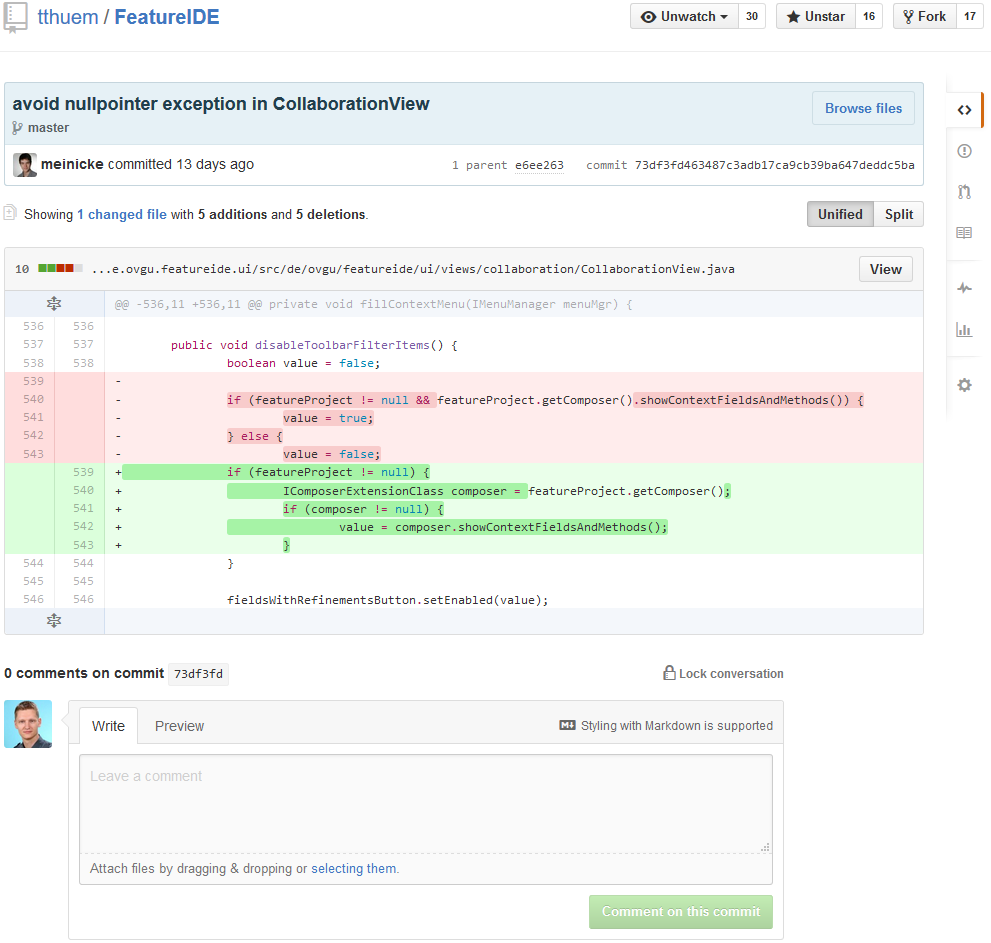
\includegraphics[height=.9\textheight]{../pics/codereview/github2}}
\end{frame}
